\subsection{Misura della lunghezza focale della lente L2}
%
    \begin{figure}[H]
    \centering
    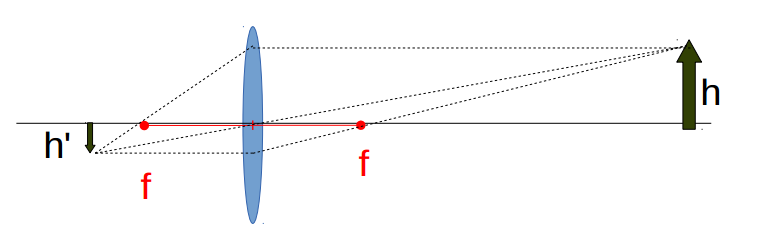
\includegraphics[scale=.4]{Grafici/O1_lente_focale.png}
    \caption{Lunghezza focale}
    \end{figure} 
%
%
Calibro illuminato da luce bianca molto intensa.\\\\
%
$p$ è la distanza calibro - lente L2;\\
$h$ è la dimensione effettiva dell'oggetto (apertura del calibro);\\
$h'$ è la dimensione dell'immagine dell'oggetto.\\
$q$ è la distanza immagine - lente L2, e si trova mediante la formula:
%
$$ \frac{h'}{h} = \frac{q}{p} $$
%
$f$ è la distanza focale della lente L2, che si ricava dalla legge dei punti coniugati:
$$ \frac{1}{p} + \frac{1}{q} = \frac{1}{f} $$
%
Ad una distanza $ p = 4610 \pm 10 $ mm, abbiamo variato l'apertura del calibro $h$ e abbiamo misurato $h'$ con il micrometro.
I dati sperimentali sono:\\
%
\begin{table}[H]
\centering
\begin{tabular}{|c|c|}
\hline
    $h$ 	&	$h'$		\\
    $mm$	&	$mm$		\\
    \hline
    10.00	&	0.60		\\
    15.00	&	0.88		\\
    18.60	&	1.07		\\
    20.00	&	1.14		\\
    25.00	&	1.43		\\
    30.00	&	1.69		\\
    35.00	&	2.00		\\
    40.00	&	2.31		\\
    45.00	&	2.59		\\
    50.00	&	2.83		\\
\hline    
\end{tabular}
\end{table}
%
Assumendo un errore di $0.02$ mm per $h'$, mediante propagazione errori e media pesata si ottiene:
$$ f = 249 \pm 1 \mathrm{ mm}$$
Valore nominale di 252 mm, ma incertezza sconosciuta.



